\documentclass[12pt]{article}
 
\usepackage[margin=1in]{geometry} 
\usepackage{amsmath,amsthm,amssymb,mathtools}
\usepackage{graphicx}
\usepackage{listings}
\usepackage{verbatim}
\usepackage{epstopdf}
\usepackage{subcaption}
\usepackage{slashbox,pict2e}
\newcommand{\N}{\mathbb{N}}
\newcommand{\Z}{\mathbb{Z}}
\graphicspath{{figures/}}
 
\newenvironment{theorem}[2][Theorem]{\begin{trivlist}
\item[\hskip \labelsep {\bfseries #1}\hskip \labelsep {\bfseries #2.}]}{\end{trivlist}}
\newenvironment{lemma}[2][Lemma]{\begin{trivlist}
\item[\hskip \labelsep {\bfseries #1}\hskip \labelsep {\bfseries #2.}]}{\end{trivlist}}
\newenvironment{exercise}[2][Exercise]{\begin{trivlist}
\item[\hskip \labelsep {\bfseries #1}\hskip \labelsep {\bfseries #2.}]}{\end{trivlist}}
\newenvironment{reflection}[2][Reflection]{\begin{trivlist}
\item[\hskip \labelsep {\bfseries #1}\hskip \labelsep {\bfseries #2.}]}{\end{trivlist}}
\newenvironment{proposition}[2][Proposition]{\begin{trivlist}
\item[\hskip \labelsep {\bfseries #1}\hskip \labelsep {\bfseries #2.}]}{\end{trivlist}}
\newenvironment{corollary}[2][Corollary]{\begin{trivlist}
\item[\hskip \labelsep {\bfseries #1}\hskip \labelsep {\bfseries #2.}]}{\end{trivlist}}
 
\begin{document}
\begin{flushright}
	EE 232E Project1 \\
	Zhiyuan Cao \\
	304397496   \\
	05/16/2017  
\end{flushright}	
\subsection*{T3.18}
\subsubsection*{(a)}
\paragraph{}
Define $g(t) =f(Z+tV)$ and restrict $g$ to the interval of values of $t$ for which $Z +tV \succ 0$. We have
\begin{align*}
&g(t) =\textbf{tr}( (Z+tV)^{-1}) \\
&\quad \ \ = \textbf{tr}((Z^{1/2}(I+tZ^{-1/2}VZ^{-1/2})Z^{1/2})^{-1}) \\
&\quad \ \ = \textbf{tr}(Z^{-1}(I+tZ^{-1/2}VZ^{-1/2})^{-1}) \\
&\quad \ \ = \textbf{tr}(Z^{-1}(I+tQ\Lambda Q^T)^{-1}) \\
&\quad \ \ = \textbf{tr}(Q^TZ^{-1}Q(I+t\Lambda)^{-1})  \\
&\quad \ \ = \sum_{i=1}^{n}(Q^TZ^{-1}Q)_{ii}(1+t\lambda_i)^{-1}
\end{align*}
\paragraph{}
Where we had $Z^{-1/2}VZ^{-1/2} = Q\Lambda Q^T$. $g(t)$ can be seen as a positive weighted sum of convex functions $1/(1+t\lambda_i)^{-1}$ and therefore is convex.
\subsection*{Problem 2}
\subsubsection*{(a)}
\paragraph{}
This is the same as hw1 and is realized by $barabasi.games()$.
\subsubsection*{(b)}
\paragraph{}
Figure \ref{fig:b1} presents the results of such random walk.
\begin{figure}[h]
	\centering
	\begin{subfigure}{.5\textwidth}
		\centering
		\includegraphics[width=.9\linewidth]{hw2p2b1.png}
		\caption{Mean}
	\end{subfigure}%
	\begin{subfigure}{.5\textwidth}
		\centering
		\includegraphics[width=.9\linewidth]{hw2p2b2.png}
		\caption{Standard Deviation}
	\end{subfigure}
	\caption{Distance $\langle s(t)\rangle$, with $n = 1000,\ t = 50,\ num\_walkers = 2000$}
	\label{fig:b1}
\end{figure}

\begin{figure}[h!]
	\centering
	\begin{subfigure}{.5\textwidth}
		\centering
		\includegraphics[width=.9\linewidth]{hw2p2b3.png}
		\caption{Mean}
	\end{subfigure}%
	\begin{subfigure}{.5\textwidth}
		\centering
		\includegraphics[width=.9\linewidth]{hw2p2b4.png}
		\caption{Standard Deviation}
	\end{subfigure}
	\caption{Distance $\langle s(t)\rangle$, with $n = 100,\ t = 50,\ num\_walkers = 200$}
	\label{fig:b2}
\end{figure}

\begin{figure}[h!]
	\centering
	\begin{subfigure}{.5\textwidth}
		\centering
		\includegraphics[width=.9\linewidth]{hw2p2b5.png}
		\caption{Mean}
	\end{subfigure}%
	\begin{subfigure}{.5\textwidth}
		\centering
		\includegraphics[width=.9\linewidth]{hw2p2b6.png}
		\caption{Standard Deviation}
	\end{subfigure}
	\caption{Distance $\langle s(t)\rangle$, with $n = 10000,\ t = 50,\ num\_walkers = 2000$}
	\label{fig:b3}
\end{figure}

\subsubsection*{(c)}
\paragraph{}
This again shares no similarity to d-dimensional random walk. Essentially the walker behave similarly to the walker in question 1. Refer to (d) for a more detailed comparison
\subsubsection*{(d)}
\paragraph{}
Figure \ref{fig:b2} and \ref{fig:b3} presents the case of $n = 100$ and $n = 10000$. As a typical realization, diameter of $n = 100, 1000$ and 10000 are $d = 12, 20$ and 28 respectively. Here the diameter again provides some sort of an upper-bound and the larger the diameter, the larger the mean and standard deviation will be.
\paragraph{}
Essentially, a random graph generated by $barabasi.games()$ has fewer high-degree nodes as compared to $erdos.renyi.games()$ where degrees are more evenly distributed. This results in mean and standard deviation converging in a much longer step. Figure \ref{fig:b4} presents such an idea. With $t=2000$ and $num\_walkers =10$ (with limited computing power we selected 10 to illustrate the concept), the mean and standard deviation are, again, bounded eventually.

\begin{figure}[h!]
	\centering
	\begin{subfigure}{.5\textwidth}
		\centering
		\includegraphics[width=.9\linewidth]{hw2p2b7.png}
		\caption{Mean}
	\end{subfigure}%
	\begin{subfigure}{.5\textwidth}
		\centering
		\includegraphics[width=.9\linewidth]{hw2p2b8.png}
		\caption{Standard Deviation}
	\end{subfigure}
	\caption{Distance $\langle s(t)\rangle$, with $n = 1000,\ t = 2000,\ num\_walkers = 10$}
	\label{fig:b4}
\end{figure}

\subsubsection*{(e)}
\paragraph{}
Again, with long enough step the walker will be trapped in clusters with high degree nodes. This is shown in Figure \ref{fig:b5}


\begin{figure} [h!]
	\centering
	\includegraphics[scale=0.7]{hw2p2edeg.png}
	\caption{Degree distribution, with $n = 1000,\ t = 50,\ num\_walkers = 200$}
	\label{fig:b5}
\end{figure}
\subsection*{Problem 3}
\paragraph{}
With the built-in function from \textit{igraph} we found the minimum spanning tree (MST), and colored each vertex by its sector. This is shown in Figure \ref{fig:03mst}. A clear trend can be observed from graph is stocks (nodes) belonging to the same sector tend to be connected, or form clusters. Recalled our computation of edge weight $d_{ij}$ from correlation coefficient $\rho_{ij}$. Since $\rho \in [-1, 1]$, The higher the correlation coefficient, the less the edge weight. Therefore, when computing MST, edges with low correlation are truncated and what is left are edges with high correlation coefficient. This can be explained as different stocks belonging to the same sector, to a certain extend, pertain a section-wise pattern. For example, investment behavior tend to be affected by the same economic/political factors, or investors in the same sector tend to play with similar strategies.

\begin{figure}[h!]
	\centering
	\includegraphics[width=.5\linewidth]{03mst.png}
	\caption{MST by Day}	
	\label{fig:03mst} 
\end{figure}


\subsubsection*{Problem 4}
\paragraph{}
\vspace{-18pt}
\begin{enumerate}
	\item If the optimal solution is unique
	\vspace{-18pt}
	\paragraph{}
	This problem is trivial since the max-flow solution is the solution with minimum penalty.
	\item If the optimal solution is not unique
	\vspace{-18pt}
	\paragraph{}
	To acquire a max-flow solution that also has the minimum penalty, we could first solve the max-flow problem with optimal value $p^{\star}$. Then we solve the following LP:
	\begin{align*}
	& minimize \quad \ \ \  \sum p_ef_e\\
	& subject \ to \qquad f_{ij} \leq c_{ij}, \ \forall (i,j) \in E\\
	&\qquad \qquad \qquad  \sum_{j:(i, j)\in E} f_{ij} - \sum_{k:(i, k)\in E} f_{jk} \leq 0, \ \forall i \in V \\
	&\qquad \qquad \qquad  f_{i, j} \geq 0, \forall (i, j) \in E\\
	&\qquad \qquad \qquad  \sum_{i:(s, i)\in E} f_{si} = p^{\star}
	\end{align*}
	\vspace{-30pt}
	\paragraph{}
	The first three constraints are exactly the same ones used in solving the max-flow problem to guarantee a same solution space. The last constraint is added to guarantee the max-flow is reached while minimizing the penalty.
\end{enumerate}

\subsection*{A4.14}
\subsubsection*{(a)}
\paragraph{}
The KKT conditions are
\begin{itemize}
	\item $x\succeq 0$, $\textbf{1}^Tx =1$,
	\item $(\nu - a_i/a^Tx-b_i/b^Tx )x_i = 0$, for $i =1,...,n$,
	\item $\nu\textbf{1} \geq a/a^Tx+b/b^Tx$
\end{itemize}
\paragraph{}
From complimentary slackness, for $x  = (1/2, 0,...,0, 1/2)$, $\nu =2$. To see optimality, $x = (1/2, 0,...,0, 1/2),\ \nu =2$ satisfies the first and second condition of KKT. To see it satisfies the last inequality,
\begin{align*}
&\nu =2 \geq a_i/a^Tx+b_i/b^Tx = \frac{2a_i}{a_1+a_n} +\frac{2b_i}{b_1+b_n} = 2\frac{a_i+a_1a_n/a_i}{a_1+a_n} \\
&\Rightarrow a_1(a_i - a_n) \geq a_i(a_i-a_n)
\end{align*}
\paragraph{}
This is follow by $a_n \leq a_i \leq a_1$ for $i=1,...,n$. Therefore $x  = (1/2, 0,...,0, 1/2)$ is indeed optimal.
\subsubsection*{(b)}
\begin{align*}
&\log(2(u^TAu)^{1/2}(u^TA^{-1}u)^{1/2}) = \log2 +\frac{1}{2}\log(z^T\Lambda z) + \frac{1}{2}\log(z^T\Lambda^{-1} z)\\
&\qquad \qquad \qquad \qquad \qquad \qquad \ \leq \log2 +\log(\frac{1}{2}a_1+\frac{1}{2}a_n) +\log(\frac{1}{2}a_1^{-1}+\frac{1}{2}a_n^{-1}) \\
&\qquad \qquad \qquad \qquad \qquad \qquad \ = \log2 +\frac{1}{2}\log(2+\frac{a_1}{a_n}+\frac{a_n}{a_1})\\
&\qquad \qquad \qquad \qquad \qquad \qquad \  =\log(\sqrt{\frac{a_n}{a_1}}+ \sqrt{\frac{a_1}{a_n}}),
\end{align*}
\paragraph{}
with first equality followed by eigendecomposition $u^TAu =u^TQ\Lambda Q^Tu$ and let $z = Q^Tu$ and second inequality followed by letting $a_k =\lambda_k$. Finally, since taking the exponential on both sides does not change the inequality, the \textit{Kantorovich inequality} holds.
\subsection*{A4.17}
\subsubsection*{(a)}
\paragraph{}
Using eigendecomposition, $A = Q\Lambda Q^T$ and \textbf{tr}$(AX) $=\textbf{tr}($\Lambda Q^TXQ$). Set $Y = Q^TXQ$ and we have,
\begin{align*}
&maximize \qquad \sum_{i=1}^{n}Y_{ii}\lambda_i\\
&subject\ to \qquad \sum_{i=1}^{n}Y_{ii} = r\\
&\qquad \qquad \qquad \ \ 0 \leq Y_{ii} \leq 1, \qquad i=1,...,n
\end{align*} 
\paragraph{}
This is followed by trace only involves the diagonal elements of matrix $Y$. Through inspection, the optimal value of this SDP is equal to $f(A)$ by taking $Y_{ii} = 1$ for $i=1,...,r$ and 0 otherwise.
\subsubsection*{(b)}
\paragraph{}
$f(A)$ is convex since it is the pointwise supremum of a family of linear function.
\subsubsection*{(c)}
\begin{align*}
&L(X, \nu, U, V) = -\textbf{tr}(AX) +\nu(\textbf{tr}X-r) - \textbf{tr}(UX) + \textbf{tr}(V(X-I))\\
&\qquad \qquad \quad \ \ 	= -\textbf{tr}((A-\nu I -U +V)X)-r\nu-\textbf{tr}V\\
&\qquad \qquad \quad \ \ =\begin{cases}
& -r\nu-\textbf{tr}V \qquad \text{if} \ -A-\nu I -U +V = 0\\
& -\infty \qquad \qquad \quad  \text{otherwise}
\end{cases}
\end{align*}
\paragraph{}
Therefore, the dual function
\begin{align*}
&maximize \qquad  -r\nu-\textbf{tr}V \\
&subject\ to \qquad A+ \nu I \preceq V\\
&\qquad \qquad \qquad  \ V \succeq 0,
\end{align*}
\paragraph{}
or in minimization form,
\begin{align*}
&minimize \qquad  r\nu+\textbf{tr}V \\
&subject\ to \qquad A+ \nu I \preceq V\\
&\qquad \qquad \qquad  \ V \succeq 0,
\end{align*}
\paragraph{}
Through strong duality, this optimal value of this SDP equals to $f(A(x))$.
\subsubsection*{A3.17}
\paragraph{}
See Figure 1 and M-code
\begin{figure}
	\centering
	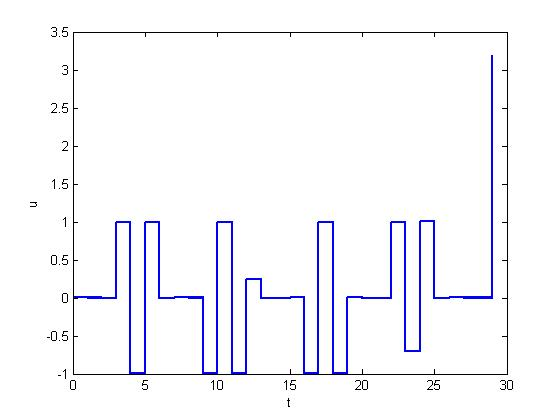
\includegraphics[scale=0.5]{fule}
	\caption{Output $u(t)$}
\end{figure}
\verbatiminput{main.m}
\section*{Conclusion}
\paragraph{}
In this report, we present analysis of network structure of a combined Facebook network and 100+ separate Google Plus networks. We conclude that \textit{Walktrap} tend to be the algorithm to deal with partitioning communities in social network, as it tend to have more smaller clusters. For Gplus network, we discovered that \textit{Infomap} tend to be the better choice over \textit{Walktrap} to discover overlaps between communities and circles. The property of \textit{Walktrap} discussed above becomes a weak point as the communities are too scattered apart. All in all, we gained a deep understanding for what kind of tools we need for specific tasks. And on the high level idea, we also learnt that for different task of analysis we need to select tools selectively.

\begin{thebibliography}{1}
	\bibitem{imdb} 
	\textit{IMDB Top 250}. May 2017,
	\text{url: http://www.imdb.com/chart/top}. 
\end{thebibliography}


\end{document}	